\begin{question}
\noindent A space observatory has a telescope mounting platform designed as a cuboid base $ABCD$--$EFGH$, used to keep a telescope perfectly stable while tracking objects in orbit.

\noindent The base $ABCD$ is horizontal, with $AB = 12$ m and $BC = 9$ m. The vertical support struts have height $AE = BF = CG = DH = 5$ m.

\noindent A control cable runs in a straight line from $H$ down to the corner $B$, as shown in the diagram.

\begin{center}
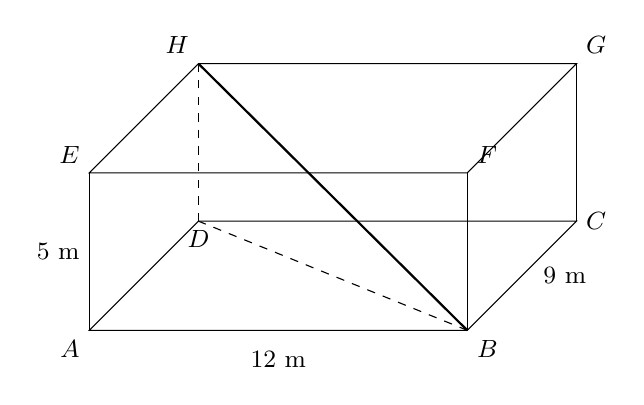
\begin{tikzpicture}[scale=1, transform shape]
    % Define the points of the cuboid: base ABCD, top EFGH
    % AB = 12, BC = 9, height = 5, scaled down for drawing (x0.4)
    \coordinate (A) at (0,0,0);
    \coordinate (B) at (4.8,0,0);
    \coordinate (C) at (4.8,0,-3.6);
    \coordinate (D) at (0,0,-3.6);
    \coordinate (E) at (0,2,0);
    \coordinate (F) at (4.8,2,0);
    \coordinate (G) at (4.8,2,-3.6);
    \coordinate (H) at (0,2,-3.6);

    % Draw the visible edges
    \draw (A) -- (B) -- (C) -- (D) -- cycle; % bottom face
    \draw (E) -- (F) -- (G) -- (H) -- cycle; % top face
    \draw (A) -- (E);
    \draw (B) -- (F);
    \draw (C) -- (G);
    \draw[dashed] (D) -- (H);

    % Diagonal of base from B to D (hidden, dashed)
    \draw[dashed] (B) -- (D);

    % Cable from H to B
    \draw[thick] (H) -- (B);

    % Labels
    \node at (A) [below left,font=\small] {$A$};
    \node at (B) [below right,font=\small] {$B$};
    \node at (C) [right,font=\small] {$C$};
    \node at (D) [below,font=\small] {$D$};
    \node at (E) [above left,font=\small] {$E$};
    \node at (F) [above right,font=\small] {$F$};
    \node at (G) [above right,font=\small] {$G$};
    \node at (H) [above left,font=\small] {$H$};

    % Side length labels
    \node at (2.4,-0.15,0) [below,font=\small] {$12$ m};
    \node at (4.95,0,-1.8) [right,font=\small] {$9$ m};
    \node at (0,1,0) [left,font=\small] {$5$ m};
\end{tikzpicture}
\end{center}

\begin{enumerate}
    \item[(a)] Calculate the length of the cable $HB$.

    Give your answer correct to 3 significant figures.

    \vspace{4.5cm}
    \answerunit{m}{3}

    \item[(b)] Calculate the angle that the cable $HB$ makes with the horizontal base plane $ABCD$.

    Give your answer correct to 1 decimal place.

    \vspace{4.5cm}
    \answerequnit{\theta}{$^\circ$}{3}
\end{enumerate}
\end{question}
